% !TeX TXS-program:compile = txs:///arara
% arara: lualatex: {shell: no, synctex: no, interaction: batchmode}

\documentclass[12pt]{article}
\usepackage[Weight=Light,math-style=french,bold-style=ISO,StylisticSet={},RawFeature={+dlig;+ordn;+zero}]{pennstander-otf}
\usepackage{tkz-tab}


\begin{document}

abcdefghijklmnopqrstuvwxyz0123456789$0123456789$

ABCDEFGHIJKLMNOPQRSTUVWXYZ

$\mathcal{abcdefghijklmnopqrstuvwxyz}$

$\mathcal{ABCDEFGHIJKLMNOPQRSTUVWXYZ}$

$\mathbb{abcdefghijklmnopqrstuvwxyz}$

$\mathbb{ABCDEFGHIJKLMNOPQRSTUVWXYZ}$

$\mathfrak{abcdefghijklmnopqrstuvwxyz}$

$\mathfrak{ABCDEFGHIJKLMNOPQRSTUVWXYZ}$

$x^{2}+y_{2}=\dfrac{1}{z}$

ffi ffl No.0123456789 BB EE

Here is some {\bfseries bold}, some {\itshape italics} and some {\bfseries\itshape bolditalics} and an equation

\[ \int_A^B f'(x)\,\text{d}x = f(B) - f(A) \]

$t = \frac{1}{4}$ or $\dfrac{1}{4}$ or $\tfrac{1}{4} \leq \tfrac{1}{3}$ or $z \in \mathbb{C}$ or $ x \in \left]0;3\right[ \cup \left[5;+\infty\right[$

$M_{2}^{10}$ or $M = \begin{pmatrix} 1&2\\3&4 \end{pmatrix}$

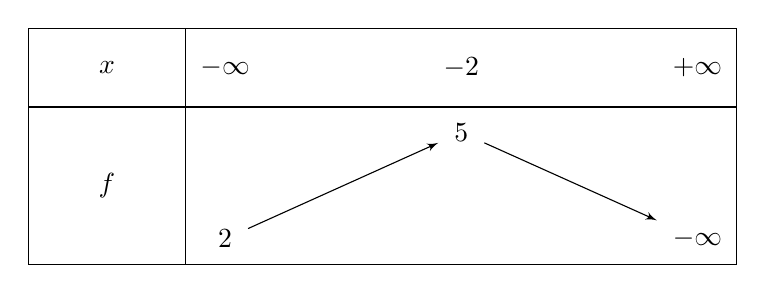
\begin{tikzpicture}
	\tkzTabInit{$x$/1,$f$/2}{$-\infty$,$-2$,$+\infty$}
	\tkzTabVar{-/$2$,+/$5$,-/$-\infty$}
\end{tikzpicture}

$\mathcal{C}_f$ ou $C_f$ ou $\mathbb{C}_{f}$ ou $\mathfrak{C}_f$

\end{document}